\chapter{Etat de l'art}
\par
La première étape de mon stage consiste à créer un module de reconstruction 3D dans le framework SolAR. Ce module est très complexe et demanderait énormément de travail et de temps pour pouvoir être créer à partir de zéro. On va donc chercher un logiciel sous licence libre afin de pouvoir l'utiliser et/ou le modifier si besoin. Afin de trouver le logiciel le plus adapté à notre utilisation, on va faire un état de l'art de différents logiciels de reconstruction 3D. 

\section{Préparatifs}

% Présentation des datasets utilisés (nb images, taille image, insideout/outside in)
Afin de pouvoir tester les différents programme de l'état de l'art, il nous faut des datasets d'images. J'en ai selectionné deux avec des caractéristiques différentes : \emph{Dinosaure} et \emph{Museum} (voir image \ref{fig:dataset_exemple}). 

\begin{figure}[ht]
    \centering
    \begin{subfigure}{0.40\textwidth}
        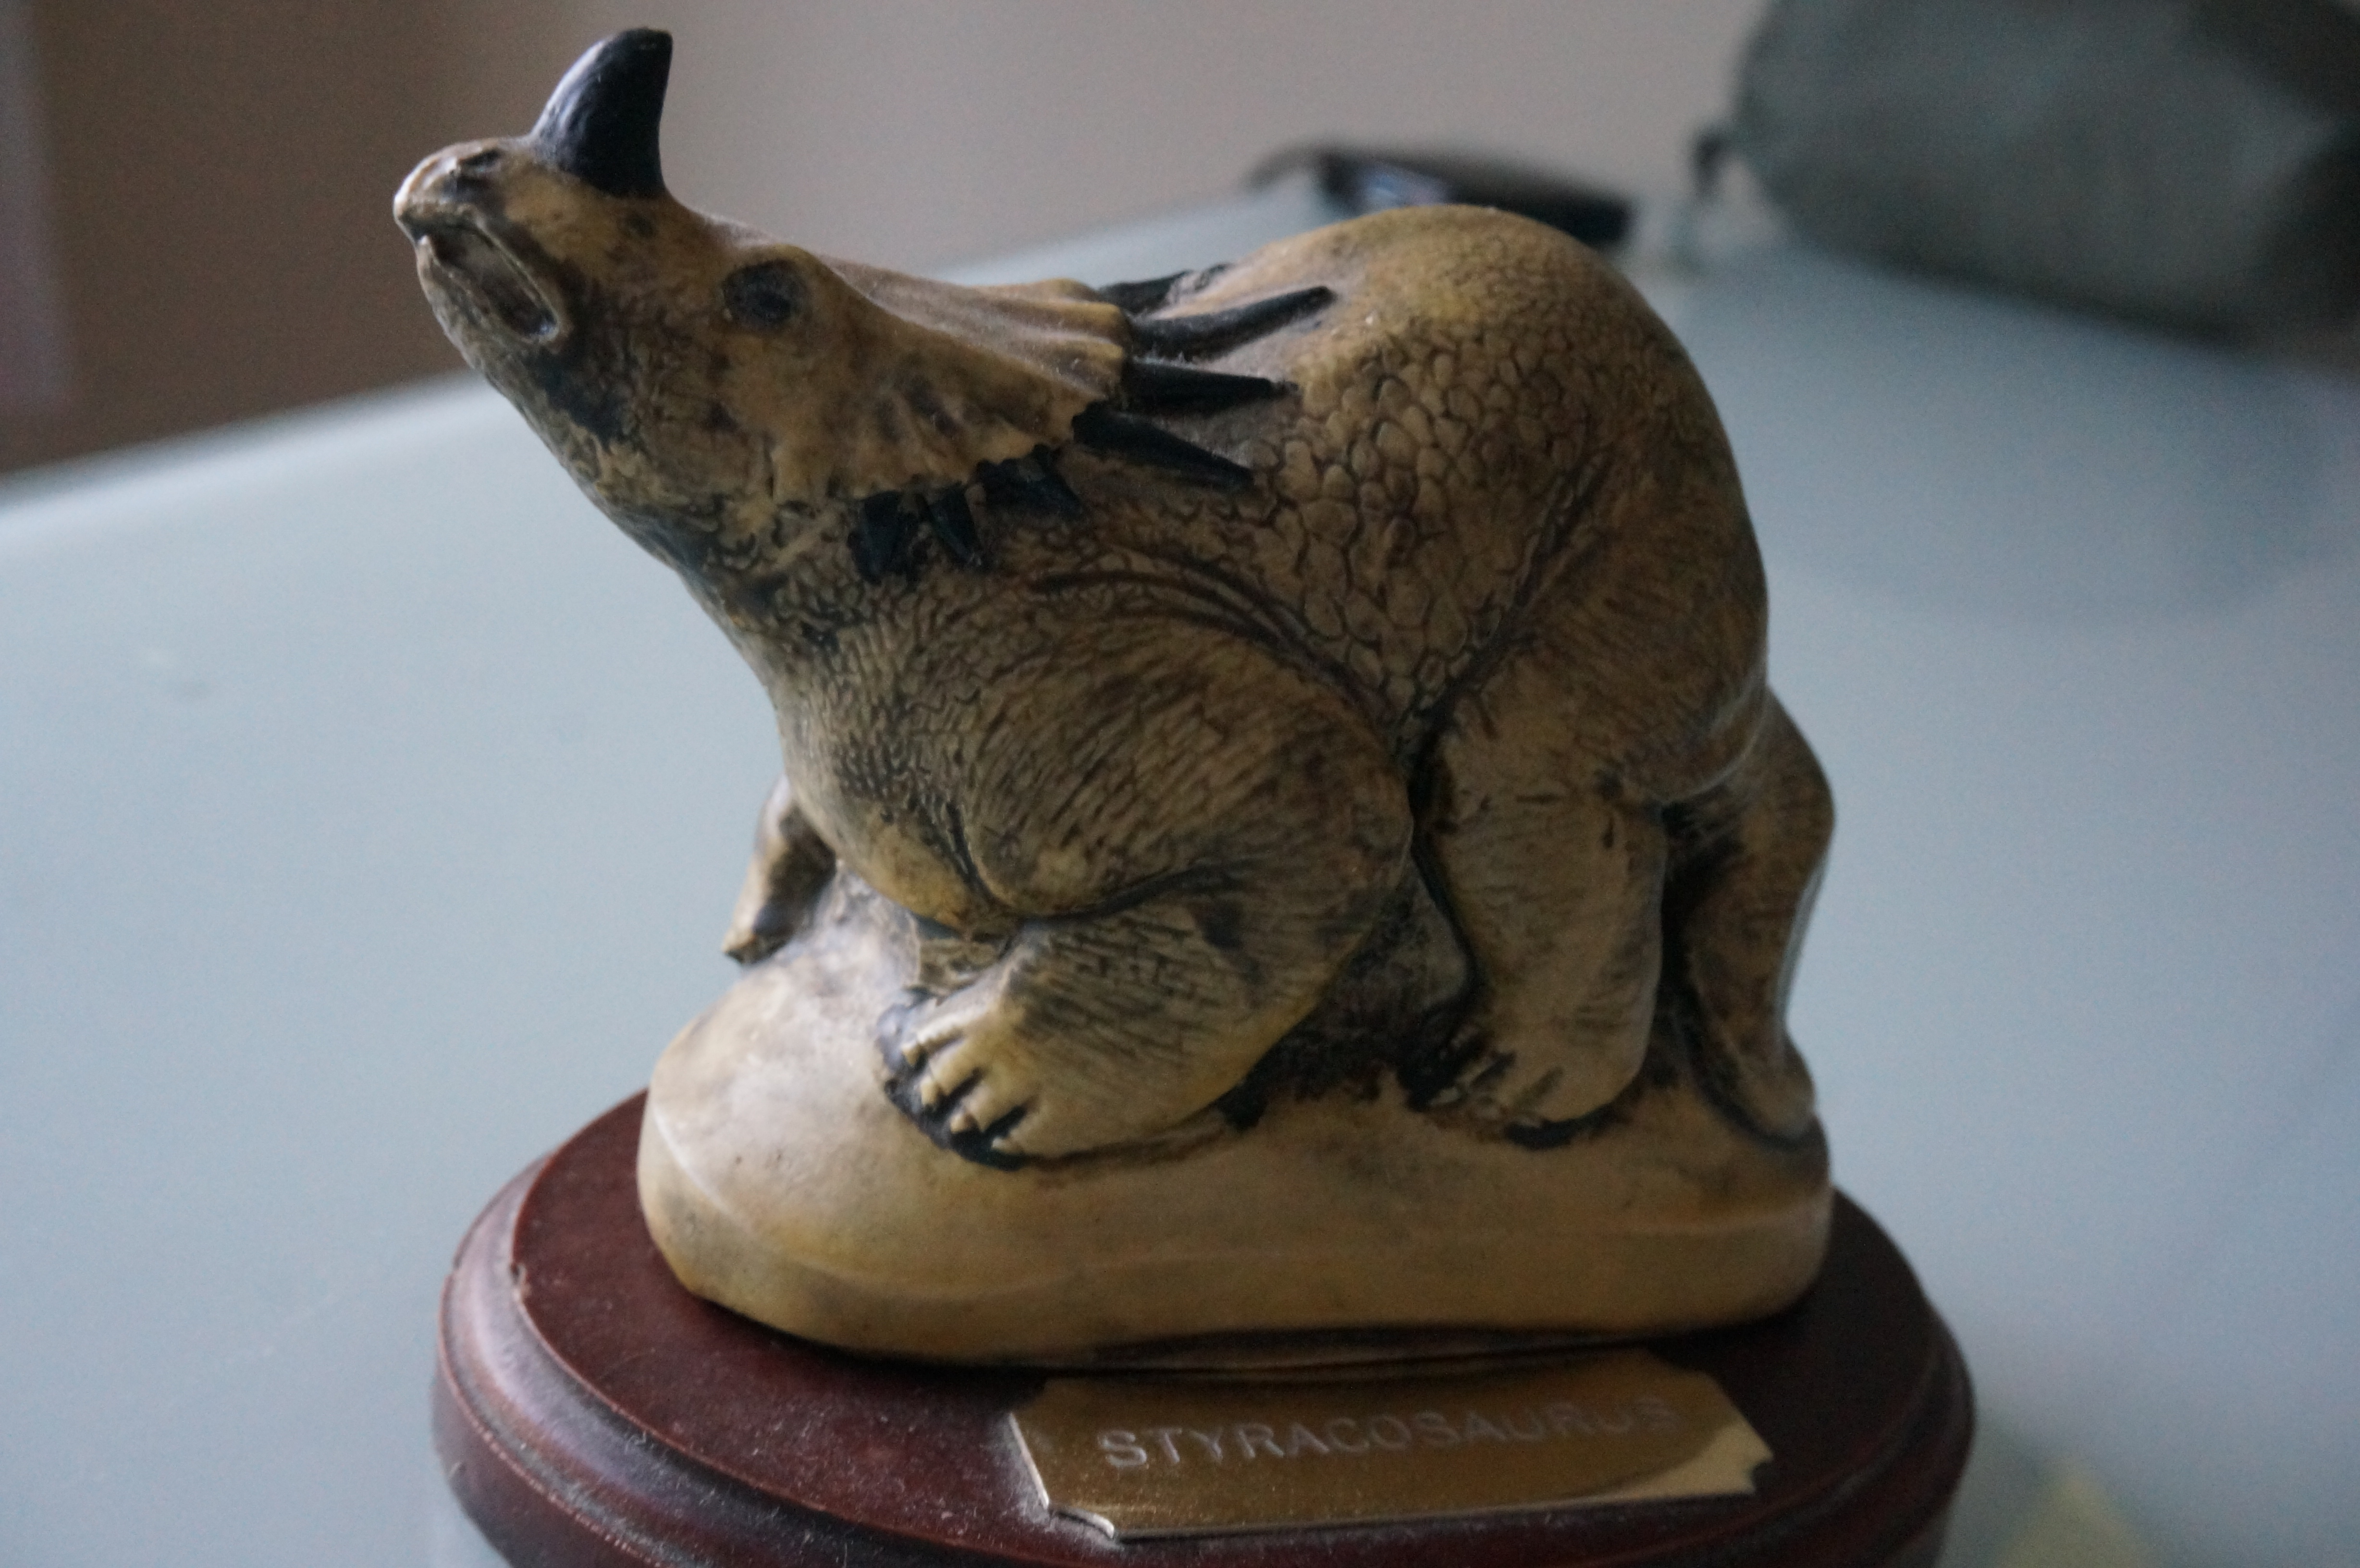
\includegraphics[width=\linewidth]{datas/dino_image.jpg}
        \caption{}
    \end{subfigure}
    \begin{subfigure}{0.47\textwidth}
        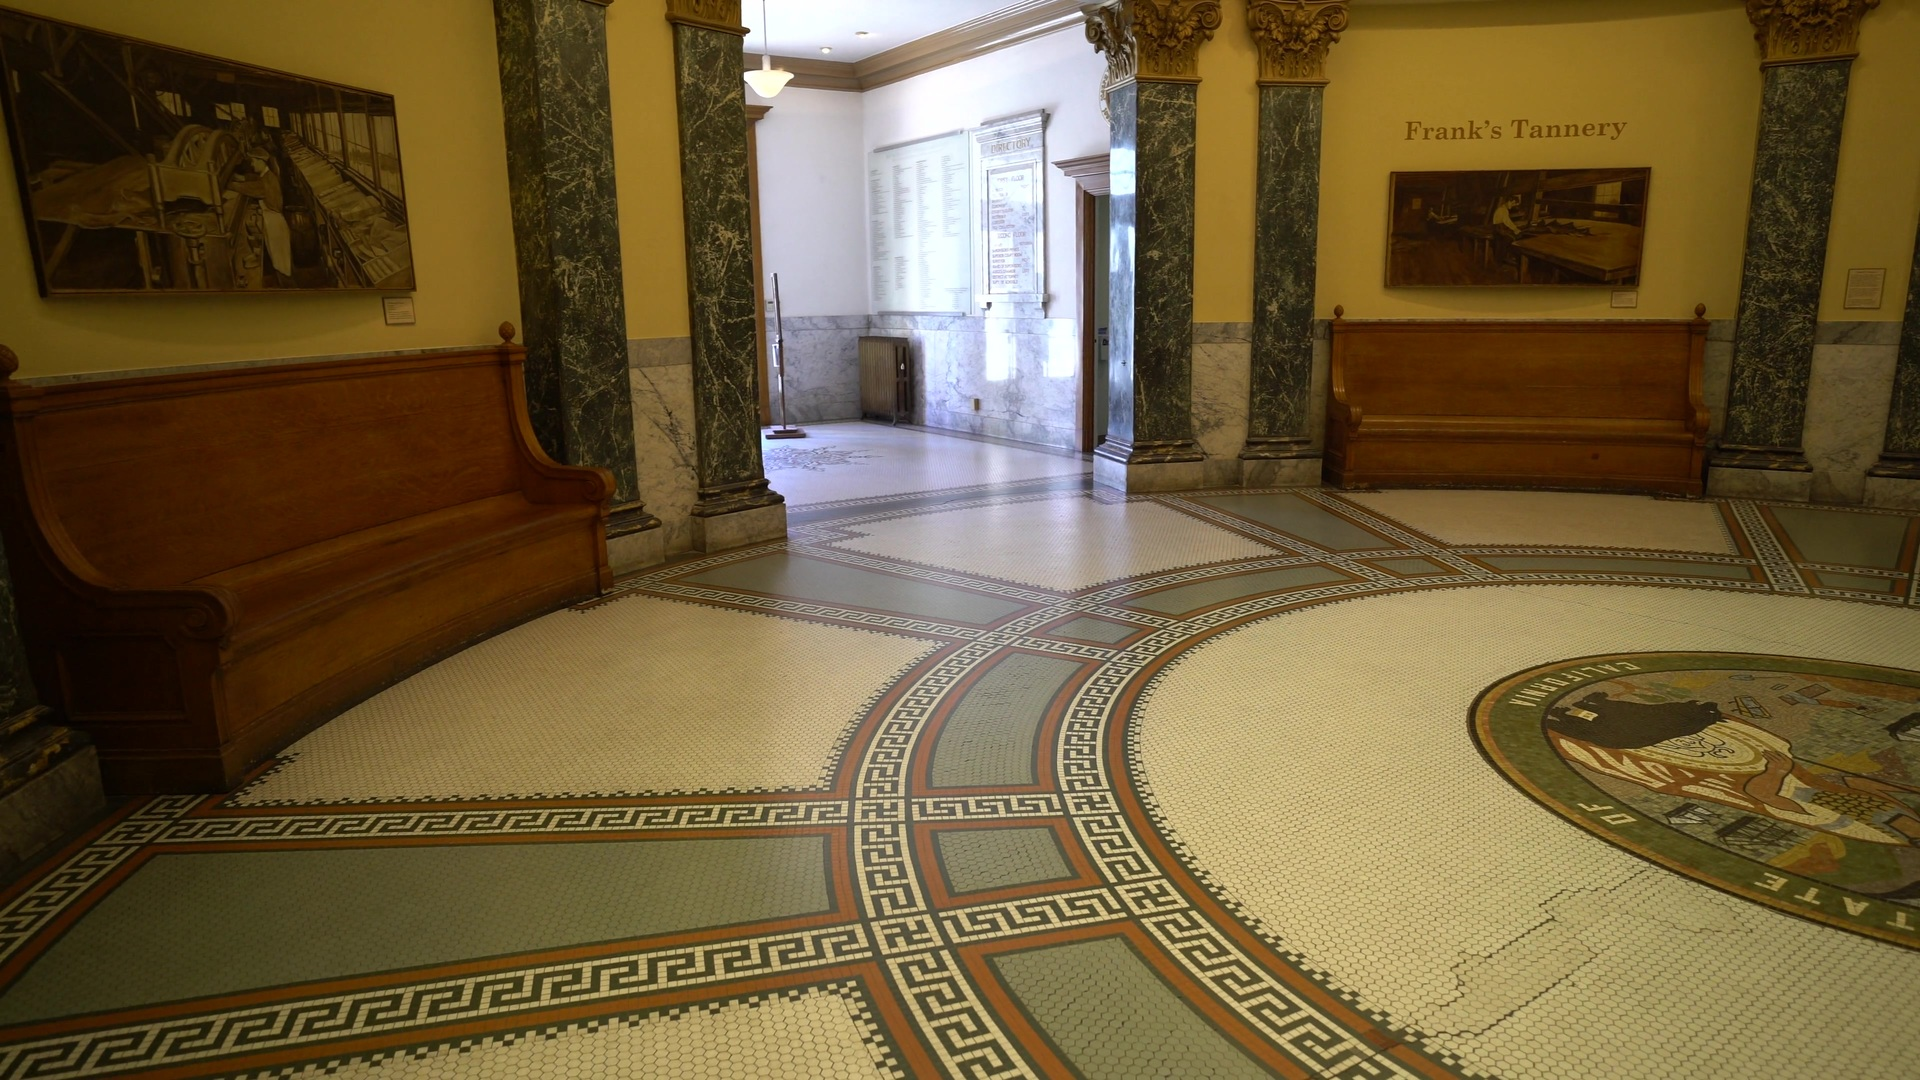
\includegraphics[width=\linewidth]{datas/museum_image.jpg}
        \caption{}
    \end{subfigure}

    \caption{Extrait du dataset \emph{Dinosaure} (a) et du dataset \emph{Museum} (b)}
    \label{fig:dataset_exemple}
\end{figure}

Le premier, une statuette de dinausaure, est composé de 53 images avec une résolution de 4912 x 3264. Celui-ci est assez léger en terme de nombre d'image est est qualifié de \emph{outside-in}, c'est-à-dire que les photos sont prises en tournant autour de l'objet. L'avantage d'avoir un petit dataset c'est d'obtenir des résultats plus rapidement car il y a moins de données à traiter. 

Le deuxième dataset, dont les photos représentent le hall d'un musée, contient 301 photos en 1920 x 1080. Celui-ci plus conséquent que le premier est \emph{outside-in} ce qui signifie qu'on est à l'intérieur de l'objet que l'on veut modéliser et que l'on prends les photos du centre vers l'extérieur. Ce critère se rapproche plus de l'objectif de SolAR qui souhaite principalement numériser des batiments. 

On utiliseras principalement le dataset Dinosaure pour gagner du temps car les logiciels sont assez chronophages. Ensuite après selection des meilleurs logiciels on pourra utiliser le dataset Museum pour appronfondir les résultats.

Pour définir quel sera le logiciel de recontruction 3D le plus adapté à SolAR on va regarder certains critères. En premier la licence des logiciels pour pouvoir avoir un maximum de liberté sur l'usage de celui-ci. Ensuite étant donné que SolAR est codé en C++, on cherche un logiciel principalement écrit dans le même langage de programmation. Enfin l'efficacité du logiciel est aussi un des critères recherchés durant cet état de l'art. Ici l'efficacité comprend la qualité du modèle 3D obtenu et la vitesse d'exécution.

\section{Présentation des logiciels}

Présentation des différents softwares
\begin{itemize}
    \item OpenSFM
    \item VisualSFM
    \item OpenMVG + OpenMVS
    \item Alicevision Meshroom
    \item Regard3D
    \item Colmap
\end{itemize}

Affichage des résultats (scene 3D : annexe \ref{fig:results_etat_art})

\addimage[0.99]{table_etat_art}{Résultats du benchmark}

\section{Choix final}

Explication du choix final

Transition vers la partie suivante